\documentclass[letterpaper, onecolumn,10pt,draftclsnofoot]{IEEEtran}
\usepackage{lipsum}
\usepackage[final]{pdfpages}
\usepackage{graphicx}
\usepackage{amssymb}
\usepackage{amsmath}
\usepackage{amsthm}

\usepackage{alltt}
\usepackage{float}
\usepackage{color}
\usepackage{url}
\usepackage{listings}
\lstset{ 
   language=C++,                % choose the language of the code
   basicstyle=\small,        % the size of the fonts that are used for the code
   keywordstyle=\color{blue},
   stringstyle=\color{red},
   commentstyle=\color{green},
   numbers=left,                   % where to put the line-numbers
   numberstyle=\footnotesize,      % the size of the fonts that are used for the line-numbers
   stepnumber=1,                   % the step between two line-numbers. If it is 1 each line will be numbered
   numbersep=5pt,                  % how far the line-numbers are from the code
   backgroundcolor=\color{white},  % choose the background color. You must add \usepackage{color}
   showspaces=false,               % show spaces adding particular underscores
   showstringspaces=false,         % underline spaces within strings
   showtabs=false,                 % show tabs within strings adding particular underscores
   frame=single,           % adds a frame around the code
   tabsize=2,          % sets default tabsize to 2 spaces
   captionpos=b,           % sets the caption-position to bottom
   breaklines=true,        % sets automatic line breaking
   breakatwhitespace=false,    % sets if automatic breaks should only happen at whitespace
   escapeinside={\%*}{*)}          % if you want to add a comment within your code
   }
   \usepackage{balance}
   \usepackage[TABBOTCAP, tight]{subfigure}
   \usepackage{enumitem}
   \usepackage{pstricks, pst-node}

   \usepackage{geometry}
   \usepackage{longtable,hyperref}
   \geometry{textheight=8.5in, textwidth=6in, margin=0.75in}
 
   \renewcommand*\rmdefault{cmr}

   \newcommand{\cred}[1]{{\color{red}#1}}
   \newcommand{\cblue}[1]{{\color{blue}#1}}
   \newcommand{\itab}[1]{\hspace{4em}\rlap{#1}}


   \title{Final Report}
   \author{Hailey Palmiter, Scott Griffy, and Ryan Kitchen}
   \date{\today}

   %% The following metadata will show up in the PDF properties
   \hypersetup{
      colorlinks = true,
      urlcolor = black,
      pdfauthor = {Palmiter, Griffy, Kitchen},
      pdftitle = {HawkEye Final Report},
      pdfsubject = {CS463},
      pdfpagemode = UseNone
   }
   \begin{document}
   \begin{titlepage}
	\centering
       	\vfill
       
	\begin{figure}[!ht] 
	\centering
	
\includegraphics[width=0.6\textwidth,natwidth=610,natheight=642]{images/HawkEye_Logo.png}  
	\end{figure}

	\vfill
	{\bfseries\Large
	 Image Processing Vision System for Manned and Unmanned Aircraft\\
	 \vskip.5cm
         CS 463 - Senior Capstone Final Report\\
         \vskip.5cm
         June 10th, 2016\\
         \vskip1cm
         Group 4 - HawkEye Crew\\ 
         \vskip.5cm
         Hailey Palmiter\\
         \vskip.5cm
         Scott Griffy\\
         \vskip.5cm
         Ryan Kitchen\\
        }
    
      \vfill
      \vskip2cm
      \begin{abstract} %Needs improvement%
	  This document is a final report constructed using the IEEEtran style guidelines. The report provides an introduction to our senior project, a project description, and a personal overview from each member of the team about what they learned over the course of the project. The report includes our original requirements document, design document, and technological review with an added discussion about each document. This discussion describes how the project has changed over the course of the year in comparison to how it was perceived during the planning process. Also included is our weekly blog posts that were been generated over the course of the year to keep our TA and our sponsors up to date with our progress. We also included our final poster that was used at the Engineering Expo. Appendix 1 covers essential code listings and appendix 2 displays the hardware we used and a few output images from our vision system. 

      \end{abstract}
      \vfill
   \end{titlepage}
   
   \onecolumn
   \tableofcontents
   \newpage
   \bigskip
\IEEEraisesectionheading{\section{Introduction}\label{sec:introduction}}
	Rockwell Collins, our project sponsor, designs video vision systems for pilots to use during flight. Pilots often use these enhanced image systems to help them see better in rough weather conditions, and to generally assist during different flight operations such as landing. An example of this functionality could be overlaying a pilot's view with graphics to help the pilot locate a landing strip in a storm or automatically turning a night-vision camera off when it is not needed in order to save power. The hardware used for this system must limit the power consumption it pulls from the aircraft, and also must be lightweight as weight is a very expensive resource on aircraft. Even an extra five pounds added to the plane during a year can add up to thousands of dollars in fuel costs. In order to provide pilots with enhanced image processing while maintaining low power consumption and low weight, Rockwell Collins develops software on Field Programmable Gate Arrays (FPGAs). While it meets the power and weight requirements, this piece of hardware makes the code very complex and very costly to develop. New vision enhancements can take weeks or months to develop on the FPGAs. The FPGAs are currently Rockwell Collins only option that meets the requirements needed to create practical systems that pilots can use effectively.\\
\par
Our goal is to provide a proof of concept for an alternative to Rockwell Collins' FPGAs. It must meet the performance metrics, provide faster implementation time, and reduce the cost of production. Specifically, we are designing a proof of concept using single board computers (SBCs). Single board computers differ from FPGAs because they have a standardized execution environment, which allows simpler code to be executed on it, reducing the development time. Single board computers also use low cost hardware and don't consume much power. If we can prove that the video quality produced by the SBCs is adequate for pilots to use, they will meet all the requirements needed to develop a practical vision system. In the air, FPGAs often take feeds from multiple cameras and run a lot of processing algorithms on those images. In order to be effective, the SBCs should also be able to handle this operation. Our project aims to test and measure the capabilities of a single board computer by delivering a multiple-stream video display that has been processed to a high degree. We believe the best candidate for this is to use NVIDIA's single board computer: the Jetson TX1. Our goal is to fully test the Jetson TX1's ability to provide enhanced imaging. This proof of concept will result in measurements that will help Rockwell Collins determine the practicality of using single board computers for their vision systems.\\
\par
   %About clients roles and who they were, team members and our roles%
Our clients are Carlo Tiana and Weston Lahr through Rockwell Collins.
The members of the HawkEyed Crew are: Scott Griffy, Hailey Palmiter, and Ryan Kitchen.
Ryan Kitchen worked on the technical side of the project. Scott helped with some of the technical side and wrote documentation. Hailey edited and wrote documentation and managed the project.
We communicated with the clients to define requirements and secure hardware necessary for the project. We also got a lot of the hardware from our instructor, Kevin McGrath.

\section{Original Requirements Document}
	\subsection{Introduction}
\subsubsection{Purpose}
Rockwell Collins currently develops their vision systems on Field Programmable Gate Arrays, making the time from design to product very long.  Rockwell Collins is considering using Single Board Computers as a way to speed up this cycle.
Our goal is to provide a proof of concept for a vision system on a Single Board Computer for Rockwell Collins. This proof of concept should help Rockwell Collins measure the practicality of Single Board Computers for vision systems.\\

\subsubsection{Scope}
Development will be limited to the Jetson TK1 or Jetson TX1. Evaluation of hardware platforms other than the TK1 and TX1 will be a stretch goal. In which case, these boards will serve as the base unit for comparison. Software shall interface to a minimum of 2 cameras, receive video, and display it on a monitor while logging metrics. Metrics will be frames per second and operations per second.\\

\subsubsection{Definitions}
\begin{description}[leftmargin=2cm,labelindent=2cm]
	\item [SBC] Single board computer
	\item [RC] Rockwell Collins
	\item [FPS] Frames per second
	\item [FPGA] Field-programmable gate array
	\item [USB] Universal serial bus
	\item [PoC] Proof of concept
	\item [SVS] Simple vision system\\
\end{description}

\subsubsection{References}
Carlo Tiana, Airborne Vision Systems Expert at Rockwell Collins
Weston Lahr, Senior Software Engineer at Rockwell Collins,
Jetson TK1 Embedded Hardware, NVIDIA\\

\subsubsection{Assumptions and Constraints}
We're assuming that either Jetson model can handle some sort of camera vision system. From initial investigations it appears that the Jetson TX1 is a likely candidate to support our project goals.

\subsection{Overall Description}
This section will give a bird's eye view of the project, outlining the major features and their purpose.\\
\subsubsection{Product Perspective}
  \paragraph{System Interfaces}
  Linux, Jetson Distro
  \paragraph{User Interfaces}
  While using our deliverable, the user should be able to view output image from the Jetson.
  \paragraph{Software Interfaces}
  Our deliverable should be a demonstrate of the Jetson's video output, charts that display capability performance, information about the complexity and amount of video processing operations. A stretch goal would include to have the same output of the software running on a second screen.
  \paragraph{Hardware Interfaces}
  We must choose an interface between our program and the chosen camera attached to the Jetson SBC. We must also interface with the relative camera processing systems on the Jetson.
  \paragraph{Communication Interfaces}
  We will communicate with at least two different camera streams, from two separate cameras attached to our SBC.\\
  
\subsubsection{Product Functions}
The delivered demonstration should accurately demonstrate the performance limitations of the Jetson TK1 or TX1. Should the timeframe allow, we are to continue investigating other SBCs and providing a similar overview of other researched SBCs.\\

\subsubsection{User Characteristics}
Our users will be RC developers, looking to implement a given filter for vision processing platforms.\\

\subsubsection{Constraints}
Our deliverable must run on either the Jetson TK1 or Jetson TX1, and should simply test the Jetson's capabilities. We will use 1080p cameras.\\

\subsubsection{Assumptions and Dependencies}
We are assuming that the Jetson can at least handle some level of video processing.We are also going to rely on libraries and the operating system provided by Nvidia for the Jetson.\\

\subsubsection{Stretch Goal Timeline}
Stretch goals defined throughout this document may be delayed until all other requirements are finished and are not required to be in the deliverable at any point.

\subsection{Specific Requirements}
This section will outline some of the more specific parts of the project along with exact requirements that the deliverable should meet.\\

\subsubsection{External Interfaces}
\begin{description}[leftmargin=2cm,labelindent=2cm]
	\item [Two 1080p Cameras] These will be used to transfer video data to the Jetson to be processed and displayed on a monitor.
	\item [Monitor] Any monitor able to adequately display the output of the chosen SBC for the purposes of evaluation. 
	\item [Jetson] Should be able to read and process video data and stream it out to a monitor.\\
\end{description}

\subsubsection{Functions}
The system shall take input from the cameras and perform as much video processing on it as possible before dipping under the 30 fps minimum.
If the system can't handle 30fps without any extra video processing, it should simply be displayed at the fastest fps possible.\\

\subsubsection{Performance Requirements}
The system should support at least 2 cameras with a stretch goal of 3 cameras.
The system should support video output on one monitor, and if possible the video should be displayed at 30fps.\\

\subsubsection{Design Constraints}
Since this is a proof of concept, the only real design constraint is that it should be able to correctly assess and demonstrate the hardware limitations of the Jetson SBC.\\

\subsubsection{Maintainability}
Maintainability, outside of our timeframe, is a low-priority requirement as we are only delivering a proof of concept for the capabilities of our SBC.\\

\subsubsection{Portability}
Our software should give some idea of how similar code would perform on other platforms, even though the PoC itself does not have to be portable. The same goes for the camera and monitor.In order to help our stretch goal of evaluating a second SBC, it would help if the code, cameras, and monitor were all collectively portable to the second platform.\\

\subsection{Stretch Goals}
Some stretch goals were listed throughout the requirements. One purpose of the stretch goals is to further increase the effectiveness of the proof of concept. These added goals further stress the limitations of the Jetson TK1 or TX1, to further expand the capabilities of these SBC. A few other stretch goals not mention above would be implementing the same system on a similar SBC, and comparing that with the Jetson TK1 or TX1, or implementing object tracking as a video processing operation to test performance of the SBCs.\\

\subsection{Gantt Chart}
\begin{figure}[H] 
\centering
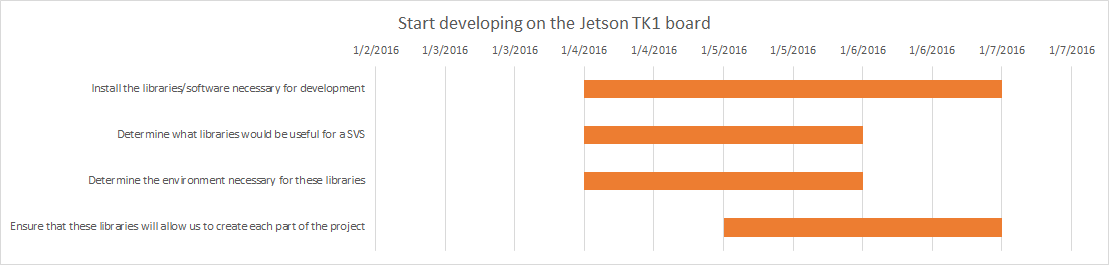
\includegraphics[width=1.0\textwidth,natwidth=1210,natheight=642]{gantt/original/starting.png}  
\end{figure}
\begin{figure}[H] 
\centering
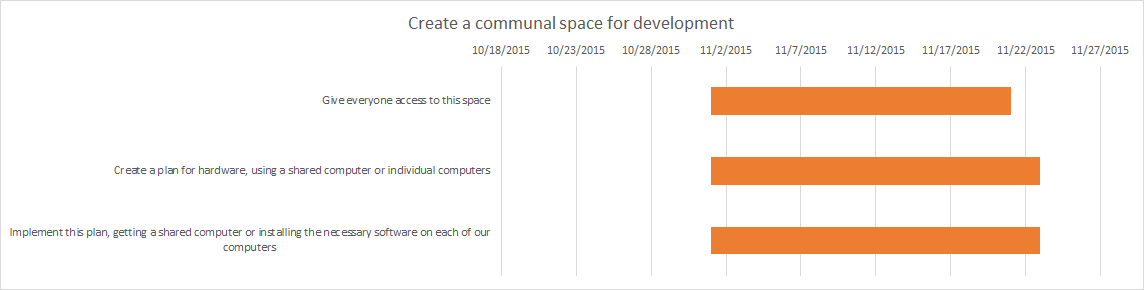
\includegraphics[width=1.0\textwidth,natwidth=1210,natheight=642]{gantt/original/communal.png}  
\end{figure}
\begin{figure}[H] 
\centering
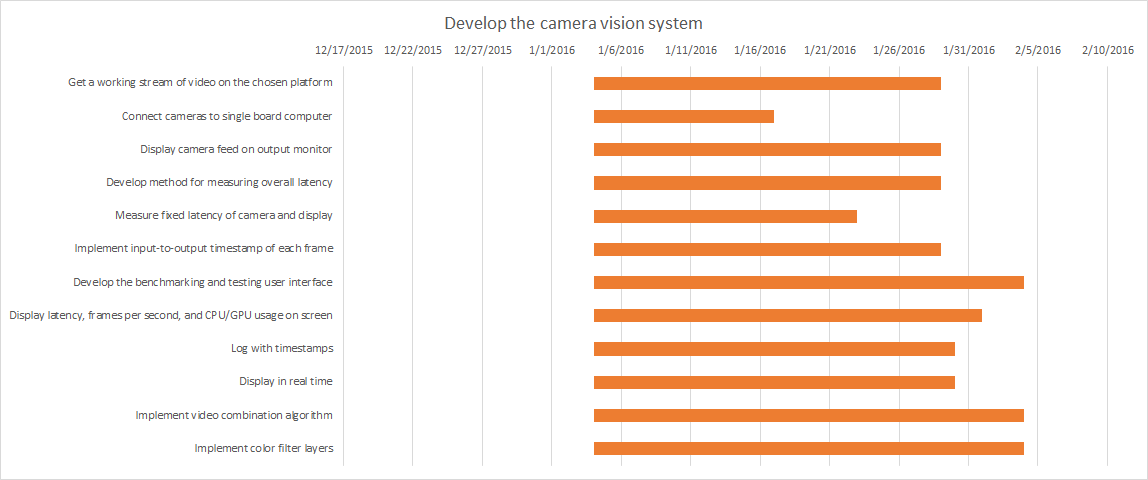
\includegraphics[width=1.0\textwidth,natwidth=1210,natheight=642]{gantt/original/develop.png}  
\end{figure}
\begin{figure}[H] 
\centering
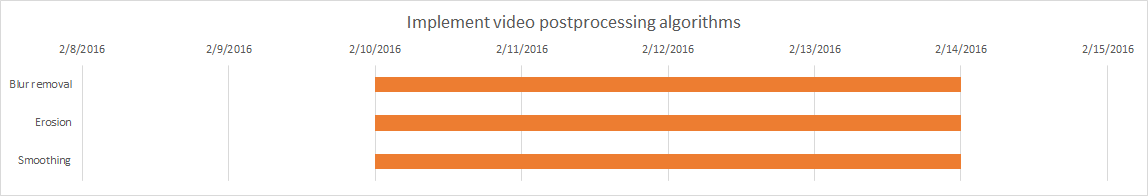
\includegraphics[width=1.0\textwidth,natwidth=1210,natheight=642]{gantt/original/algos.png}  
\end{figure}
\begin{figure}[H] 
\centering
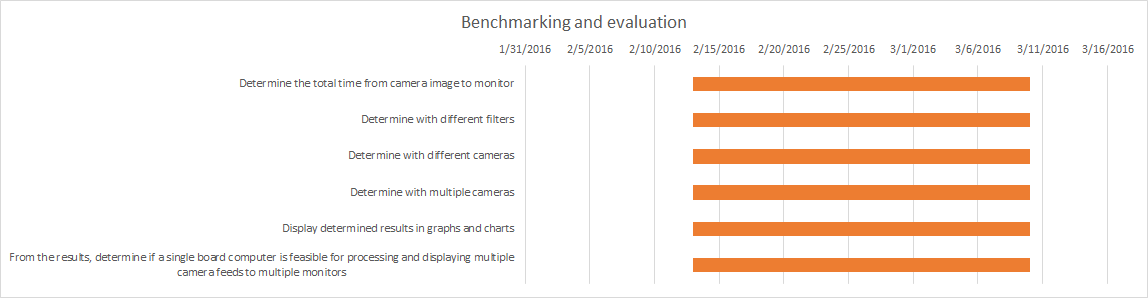
\includegraphics[width=1.0\textwidth,natwidth=1210,natheight=642]{gantt/original/eval.png}  
\end{figure}
\begin{figure}[H] 
\centering
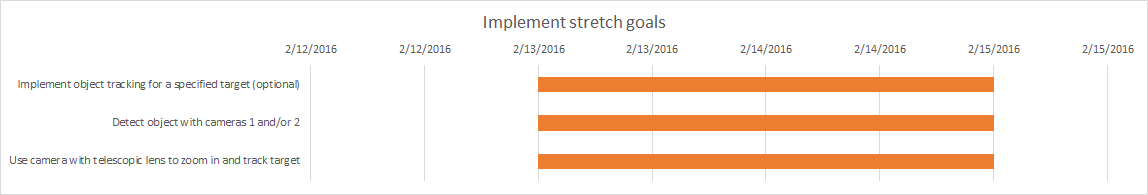
\includegraphics[width=1.0\textwidth,natwidth=1210,natheight=642]{gantt/original/stretch_goals.png}  
\end{figure}



\section{Requirements Document Changes}
%Chart of changes - What new requirements were added? What existing requirements were changed? What existing requirements were deleted? Why?%
\subsection{Final Gantt Chart}

\section{Design Document}
	\subsection{Introduction}
\subsubsection{Scope}
This software will implement a framework to develop, test, and benchmark video processing
algorithms. The users will be able to test different combinations of algorithms using one or multiple
camera inputs and produce output to one or multiple display windows. This software will be used by
HawkEye Crew to determine if the Nvidia Jetson TK1 or other off the shelf single board computers have
high enough performance to replace FPGA-based video processing systems currently used by Rockwell
Collins.\\
\subsubsection{Purpose}
This software description document will provide HawkEye Crew with a road map to complete
development of the software and fulfill the requirements in our Software Requirements Specification.
This document explains how the system is going to work, who is going to use it, and how it is meant to
be used.\\
\subsubsection{Intended Audience}
The intended audience of this design document is the developers who will design the system \(us\)
and the sponsors of this project at Rockwell Collins.\\
\subsubsection{References}
IEEE. IEEE Std 1016-2009 IEEE Standard for Information Technology \- System Design \- Software
Design Descriptions. IEEE Computer Society, 2009

\subsection{Definitions}
\begin{description}[leftmargin=2cm,labelindent=2cm]
	\item [SBC] Single board computer
	\item [RC] Rockwell Collins
	\item [FPS] Frames per second
	\item [FPGA] Field-programmable gate array
	\item [USB] Universal serial bus
	\item [PoC] Proof of concept
	\item [UML] Unified Modeling Language
	\item [DFD] Data Flow Diagram: Shows how data moves between different components in the system
	\item [ER Diagram] Entity Relationship Diagram: Shows how different data structures within the software are connected to each other
	\item [SDD] Software Design Description
	\item [SRS] Software Requirements Specification
	\item [SVS] Simple Vision System
	\item [YUV] A color space typically used as part of a color image pipeline
	\item [JSON] JavaScript Object Notation
	\item [Modular Video Processing System] The HawkEye Video Processing System's internal video processing algorithm management and execution system.\\
\end{description}

\subsection{Conceptual Model for Software Description}
\subsubsection{Software Design in Context}
For the HawkEye Video Processing System, we will be using a functional design method. Our
system is designed to be modular and have standardized interfaces, so we will be able to develop new
features and drop them in without modifying existing code. The reasoning for using a functional design
rather than object oriented is because our software is focused on processing individual video frames in
real time. Each algorithm instance will run once and has no state, only input and output data. For that
reason functional programming is the best choice for this design.\\

\subsubsection{Software Design Descriptions within the Life Cycle}
This document details how we are going to the implement software to meet our requirements.
During the course of development, our requirements and our SRS may be updated. This document
includes support for both our current requirements and provides room to add additional requirements.
It also adds additional operational requirements and functionality beyond those specified in the
requirements document. This document will also provide a reference for the creation of our testing plan.

\subsection{Design Architecture}
\subsubsection{Stakeholder Concerns and Requirements}
Our client Rockwell Collins would like to know if single board computers are a viable option to
implement simple vision systems on. They've enlisted us, the HawkEyeCrew, to implement a proof of
concept to measure the effectiveness of single board computers in this context.
\par
We, the HawkEye Crew, will be using this software to test various implementations of video
processing algorithms. In order for our system to be a valid proof of concept, our system will need to
meet certain performance benchmarks and functional requirements described by our SRS. Our design
concerns will be meeting these requirements.\\
\subsubsection{Description of Architectural Design}
Our system is designed to be a framework and testbed for the implementation of video
processing algorithms. This design handles the hardware input interface, video output to the monitor,
data flow between different algorithms, parallel operation of multiple operations, and benchmarking of
individual components and overall aggregate timing.
\par
In order to provide maximum flexibility and testing capabilities, the video processing algorithms and
input/output devices are built as separate, interchangeable modules. These different modules are
organized by the user in a configuration file, which determines both how the modules connect to each
other and how the log file is formatted. This enables us to track the performance of individual
algorithms and maximize our CPU and GPU usage while maintaining the performance requirements for
this project.\\
\subsubsection{Validation of Design}
The core requirements of our system that this design either implements or implements the
capability of testing are as follows:\\
\begin{enumerate}[leftmargin=2cm,labelindent=2cm]
\item System must be capable of processing multiple video streams
\item System must enable thorough testing of the Jeston's video processing capabilities
\item Frame rate must be at least 30FPS
\item End to end latency must be less than 100ms\\
\end{enumerate}

These requirements are met by the following architectural features:\\
\begin{enumerate}[leftmargin=2cm,labelindent=2cm]
\item The modular video processing system enables multiple input and output devices.
\item The modular video processing system will enable us to maximize the usage of CPU and GPU
processing power, which will show the maximum performance of the Jetson.
\item This software design includes built in speed benchmarking, so we will be able to track FPS.
\item This benchmarking system also produces latency details, so we will be able to determine if this
system is capable of meeting the latency requirements Rockwell Collins is looking for.\\
\end{enumerate}

\subsubsection{Overview of Viewpoints and Design Languages}
These viewpoints have been chosen to provide a complete description of the design and show
how the design is compliant with the SRS. Each one provides details crucial to understanding how the
design works and is a reference for implementation.\\

\begin{enumerate}[leftmargin=2cm,labelindent=2cm]
\item \textbf{Context viewpoint:}
This viewpoint shows the different potential users of the software and how they would
interact with our system.\\
Design Languages: Use Case Diagram
\item \textbf{Structure viewpoint:}
This viewpoint shows how the streaming video flows through the system, and identifies the
internal and external data connection points in the system. This viewpoint also shows the
components of the system which enable connection of cameras via USB as per the SRS.\\
Design Languages: Data Flow Diagram
\item \textbf{Interaction viewpoint:}
This viewpoint shows the order of operations on processing a video frame, as well as how
the timing is integrated to meet the performance benchmarking requirement.\\
Design Languages: UML Sequence Diagram
\item \textbf{Information viewpoint:}
This viewpoint details how the modular video processing system determines the order of
operations for the various elements and algorithms it can create. It shows how the system
meets the requirement for modularity and the capability to use multiple input and output
devices.\\
Design Languages: Entity Relationship Diagram
\item \textbf{State Dynamics Viewpoint:}
While the algorithm implementations in our design are stateless, the system itself is not.
This viewpoint shows the transitions between different states and provides a road map for
different states which will need to be individually tested.\\
Design Languages: UML State Transition Diagram
\end{enumerate}

\subsection{Design Viewpoints}
\subsubsection{Context Viewpoint}

	\paragraph{Users and Design Concerns}
	The design features in this document are chosen to create value for several different
kinds of users and stakeholders. These users interact with the software in different ways.\\
	\begin{enumerate}[leftmargin=2cm,labelindent=2cm]
    	\item \textbf{Pilot:}
	Our intended user will be a pilot of a manned or unmanned aerial vehicle. This software
	is designed to provide increased and extensible functionality for onboard camera
	systems. Because our product is a proof of concept, there won't be a real pilot, but the
	pilot has been included as a user because the application of this design is to create
	better equipment for pilot use. This pilot will be 'using' our product and needs the
	video stream to meet the requirements outlined in the SRS.
	\item \textbf{Distributor:}
	Rockwell Collins is the sponsor and primary stakeholder in this project. They will
	evaluate the product and decide where to use it. They will also decide the feasibility of
	using this design in production and whether continuing to use single board computers
	for real-time video processing is a good idea.
	\item \textbf{Implementer:}
	The implementer has to set up the simple vision system on their given hardware. Our
	proof of concept should give some notion as to how to do this and also the feasibility
	and easiness of it. The concepts demonstrated in this design document can be used on
	different hardware, not just the NVIDIA Jetson.
	\item \textbf{Algorithm Designer:}
	The algorithm designer interacts with our software in different ways than the end user
	and implementer. This user will create custom modules and link them together with our
	easy to use configuration system. This configuration should serve as a design for other
	systems.\\
	\end{enumerate}
	
	\paragraph{Use Case Diagram}
	
	\begin{minipage}{\linewidth}
		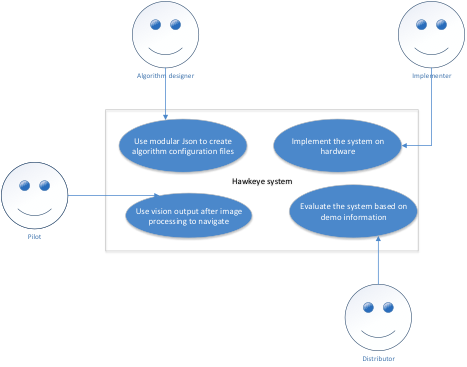
\includegraphics[keepaspectratio=true,scale=0.6]{images/UseCase_Diagram.png}
		%\begin{figure}[H] %\textwidth,natwidth=610,natheight=642
		%\centering
		%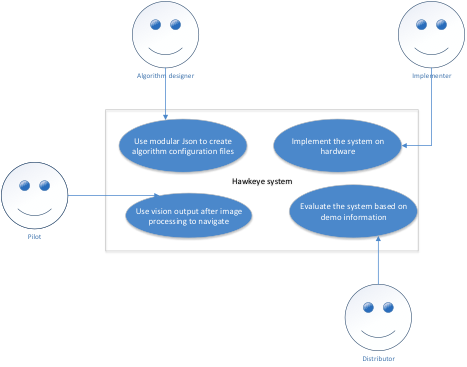
\includegraphics[width=0.6\textwidth,natwidth=610,natheight=642]{images/UseCase_Diagram.png} 
		%\caption{Use Case Diagram}\label{UseCase_Diagram.png} 
		%\end{figure}
		
	\end{minipage}
	
\subsubsection{Structure Viewpoint}
This section shows the high level organization of our software design.  
	\paragraph{Design Concerns}
	The primary design concern of this section is to show the interaction between critical components of our software design. This is valuable during implementation because it provides a reference for the required parts of the system, and also shows how the different pieces fit together.\\
	\paragraph{Design Elements}
	There are three key design elements in our software design. These elements are important because they are the basis for the entire modular video processing system.\\
	
	\begin{enumerate}[leftmargin=2cm,labelindent=2cm]
	\item \textbf{Video Buffer:}
	Shared data space provided by video4linux or created internally. Video data is in YUV format and access is provided through a void pointer to a 	contiguous block of memory.
	\item \textbf{Algorithm Module:} 
	Algorithm modules are single purpose elements that operate on one or more input buffers and provide output to one or more output buffers. They 	consist of a C function which performs the operations, and a module definition structure which provides the name and expected input and outputs 	of a module. 
	\item \textbf{Algorithm Controller:}
	This element is responsible for ordering and executing Algorithm Modules. It is the primary routine in this software design. It reads from a JSON 	configuration file, creates a module execution tree, and manages the execution of concurrently running modules.\\
	\end{enumerate}
	
	\paragraph{Structure Description}
	The HawkEye video processing software receives frames from the Video4Linux driver as a pointer to a buffer. The Algorithm Controller invokes each video processing algorithm in the order described by the configuration file, by passing them pointers to the buffers assigned to them. The video processing algorithms perform actions directly on the video buffer in order to avoid the performance hit from accessing additional memory. When the last video processing algorithm is complete, the buffer is flushed to the output device.\\
	
	\paragraph{Data Flow Diagram}
	\begin{figure}[H] 
		\centering
		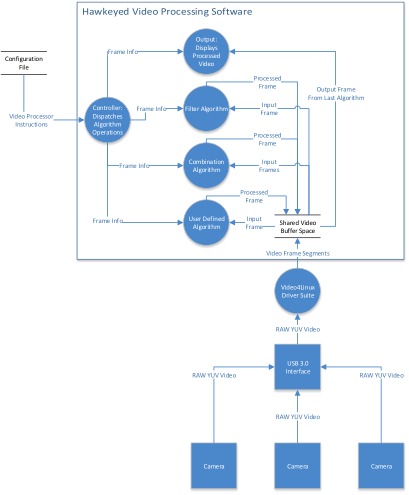
\includegraphics[width=0.6\textwidth,natwidth=610,natheight=642]{images/DataFlow_Diagram.png}  
		\end{figure}
	
\subsubsection{Interaction Viewpoint}
	\paragraph{Design Concerns}
	The main goal of this project is to determine how much video processing can be done on a SBC while maintaining a frame rate of 30 FPS and latency below 100ms. To this end, we as the user have two design concerns that need to be addressed.\\
	
	\begin{enumerate}[leftmargin=2cm,labelindent=2cm]
	\item \textbf{Latency measurement:}
	In order to keep overall latency under 100ms while maximizing the amount of processing being done, we need to know how long each algorithm 	takes to process a single frame, and also how long it takes from input to output.

	\item \textbf{FPS Monitoring:}
	Our software must process video in real time. For the purposes of this project, that has been specified as 30 FPS by our SRS. This is separate 	from the latency requirement because our system may actually be operating on multiple frames simultaneously, so the frames per second may not 	necessarily dictate the total latency.\\
	\end{enumerate}
	
	\paragraph{Design Elements}
	This viewpoint contains several design elements that depict major components of our software design.\\
	
	\begin{enumerate}[leftmargin=2cm,labelindent=2cm]
	\item \textbf{Camera Buffer:}
	Initially, camera buffer will store the data immediately loaded by the camera and will then be repurposed to hold the modified image later. This 		modified image will come from the custom algorithm code.

	\item \textbf{Custom Algorithm:}
	The custom algorithm is loaded into the system when it starts up through the JSON configuration files and dynamically linked libraries. This 		portion of the system will perform operations on the camera buffer and log the time at start and time at completion. It will then write back to the 		camera buffer, the modified image.

	\item \textbf{Log:}
	The log is a feed that will keep track of the frame rate and information about what processes are running. This should be viewable separately from 	the display.

	\item \textbf{Display:}
	The last thing that should happen when we are rendering frames is the stream to the display. This will show the final, completely processed 		image. Our client has contacted us and told us that the display should only show the video stream, not other metrics like frames per second or 		operations per frame.

	\item \textbf{Video4Linux Camera Driver:}
	This is our direct access point to the video stream from the USB camera. It enables us to receive video frames from any cameras supported by 	the Linux operating system.\\
	\end{enumerate}
	
	\paragraph{UML Sequence Diagram}
	\begin{figure}[H] 
		\centering
		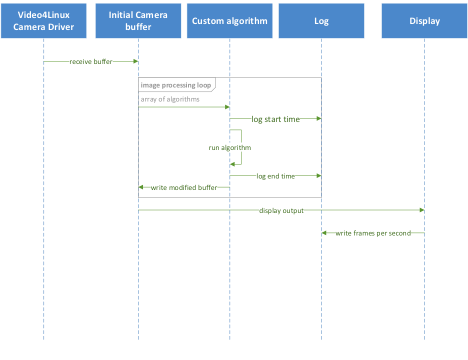
\includegraphics[width=0.6\textwidth,natwidth=610,natheight=642]{images/UML_Diagram.png}  
		\end{figure}
	
\subsubsection{Information Viewpoint}
	\paragraph{Design Concerns}
	
	\begin{enumerate}[leftmargin=2cm,labelindent=2cm]
	\item \textbf{Configuration:}
	This viewpoint addresses how the user will configure our software. It shows how the modules are connected to each other and the information that 	needs to be provided for the software to create its internal structure.

	\item \textbf{Internal Data Structure:}
	In order to implement the modular image processing system, our design needs an internal data structure in order to determine the execution path 	through the various modules.\\
	\end{enumerate}
	
	\paragraph{Design Elements}
	There are two design elements in this viewpoint:\\
	\begin{enumerate}[leftmargin=2cm,labelindent=2cm]

	\item \textbf{Module Instances:}
	Module instances are C structures that describe either input device modules, output device modules, or algorithm execution modules. They 		consist of a name, type, and the names of the connected input and output modules.
	\item \textbf{JSON Configuration File:}
	In order to create the internal data structure for our application, the user must write a configuration file in JSON format. The elements in this 		configuration file are detailed in an example below (Example JSON Configuration File).\\
	\end{enumerate}
	
	\paragraph{Description and Rationale}
	The HawkEye video processing software needs to be able to handle various configurations of multiple camera inputs and produce multiple outputs, as well as performing multiple video processing algorithms. In order to do this, it needs to know what operations to perform in what order, and where to put the data. To do this, our software uses a tree-like data structure that connects the camera inputs, algorithm modules, and outputs. An input module definition specifies what modules a camera sends data to. Each of those modules then has its own output specification, which can either go to another algorithm module or an output module. \\
	
	\paragraph{Sample Entity Relationship Diagram}
	\begin{figure}[!h] 
		\centering
		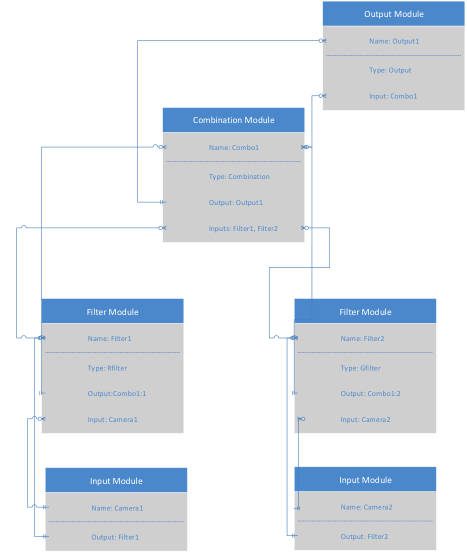
\includegraphics[width=0.6\textwidth,natwidth=610,natheight=642]{images/ER_Diagram.png}  
		\end{figure}
	
	\paragraph{Example JSON Configuration File}
	The corresponding JSON configuration file for the above ER diagram. \\
	
	 \begin{lstlisting}
	 {
   	 	"Output1":{
        			"type":"output",
        			"input":"Combo1"
    		},
    		"Combo1":{
        			"type":"Combination",
        			"inputs":"Filter1,Filter2",
        			"output":"Output1"
    		},
   		 "Filter1":{
        			"type":"Rfilter",
        			"input":"Camera1",
        			"output":"Combo1:1"
    		},
    		"Filter2":{
        			"type":"Gfilter",
        			"input":"Camera2",
        			"output":"Combo1:2"
    		},
    		"Camera1":{
       		 	"type":"Input",
        			"device":"/dev/video0",
        			"output":"Filter1"
    		},
    		"Camera2":{
        			"type":"Input",
        			"device":"/dev/video1",
        			"output":"Filter2"
   		 },
    		(not used in this example but also an option)
    		"Tracker":{
        			"type":"Module",
        			"filename":"tracker.so"
   	 	}
	}
	 \end{lstlisting}
	
	The one rule for the JSON files is that each entity must be declared before its inputs; this top down approach enables the JSON parsing algorithm to generate the module tree in a single pass. The one exception to this rule is cyclical algorithms that operate on their own output, either directly or indirectly. Support for such algorithms may be implemented, but this is not part of the current project scope. 
	
\subsubsection{State Dynamics Viewpoint}
	\paragraph{Design Concerns}
	Our program will be in multiple states while it is streaming and processing data from the camera to the display. In order to keep track of the states, we will have two state diagrams, one for the camera and a second for the software for processing.\\
	
	\paragraph{Design Elements}
	
	\begin{enumerate}[leftmargin=2cm,labelindent=2cm]
	\item \textbf{Camera:}
	For the purposes of this viewpoint, Camera shall refer to the combination of the physical camera hardware and the system level driver that exists 	outside of the HawkEye video processing application.

	\item \textbf{Software:}
	Refers to the HawkEye video processing application.\\
	\end{enumerate}
	
	\paragraph{Overview}
	The camera must be initialized before we can capture frames from it. After initialization the camera is ready for image capture. During image capture, the camera will write to a buffer on the host system. Once a frame has been written to the buffer, the software can begin image processing using the first algorithm in its configuration. When the algorithm is completed, the software will check if there is another algorithm to be performed. These two states of image processing and checking for more algorithms will loop until all algorithms have been completed. We will then write the finished image buffer to the screen. After that, we will check if the program needs to continue running or if it has received a shutdown command. To shut down we will finalize the camera, deactivate it, and stay in that state. \\
	\paragraph{States}
	
	\begin{enumerate}[leftmargin=2cm,labelindent=2cm]
	\item \textbf{Camera Initializing:}
	This is the starting state. Before we can capture frames from the camera, we must first initialize it. In this state we will also set up and synchronize the memory shared by the camera and our software.

	\item \textbf{Camera Initialized:}
	After we have initialized the camera it will be ready for capture. The software will have to start the camera's frame capture.

	\item \textbf{Camera Capturing:}
	The camera will take a moment to capture the data.

	\item \textbf{Camera Writing:} 
	The camera will have to write the data to memory. 

	\item \textbf{Image Reading:}
	Importing data from the camera's output into the software. This step should be simultaneous with camera writing as we are using the same 		memory. 

	\item \textbf{Image Processing:} 
	The image data in the buffer will be processed in place by the modular video processing system.

	\item \textbf{Process completed:}
	Once the algorithm is done operating, it will notify the controller that it has finished.

	\item \textbf{Write to Display:}
	The software will write the finalized image buffer to the display, displaying the video.

	\item \textbf{Camera Finalizing:}
	During this state, the camera is sending any remaining data and shutting down.

	\item \textbf{Camera Shut Down:}
	The camera is turned off. \\
	\end{enumerate}
	
	\paragraph{State Transition Diagram}
	Because the two state machines interact often, we have combined them in the same graphic. The following is our UML state machine:\\
	\begin{figure}[H] 
		\centering
		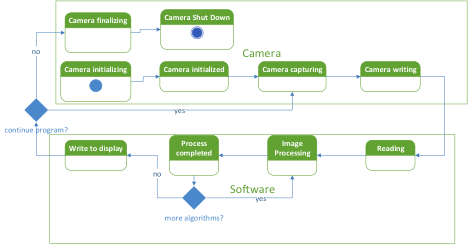
\includegraphics[width=0.6\textwidth,natwidth=610,natheight=642]{images/StateTransition_Diagram.png}  
		\end{figure}


\section{Design Document Changes}
	\subsection{Overall Description Changes}
We ended up having a physical copy of the performance of the system at expo instead of working it into our software. This was because we were advised that using the software to measure it's own performance would lead to problems, leading us to measure the performance of the system using a high speed camera which can't be done automatically.
\subsection{Specific Requirements}
One of the goals of the original design document was to create requirements that were reasonably achievable. Because of this mindset, the requirements in the document did not change very much.
\subsection{Information Viewpoint}
We had originally intended to create a modular json system, but scrapped it later on because it wasn't very valuable and created unecessary complexity.
  

\section{Technology Review}
\setlength{\fboxrule}{5pt}
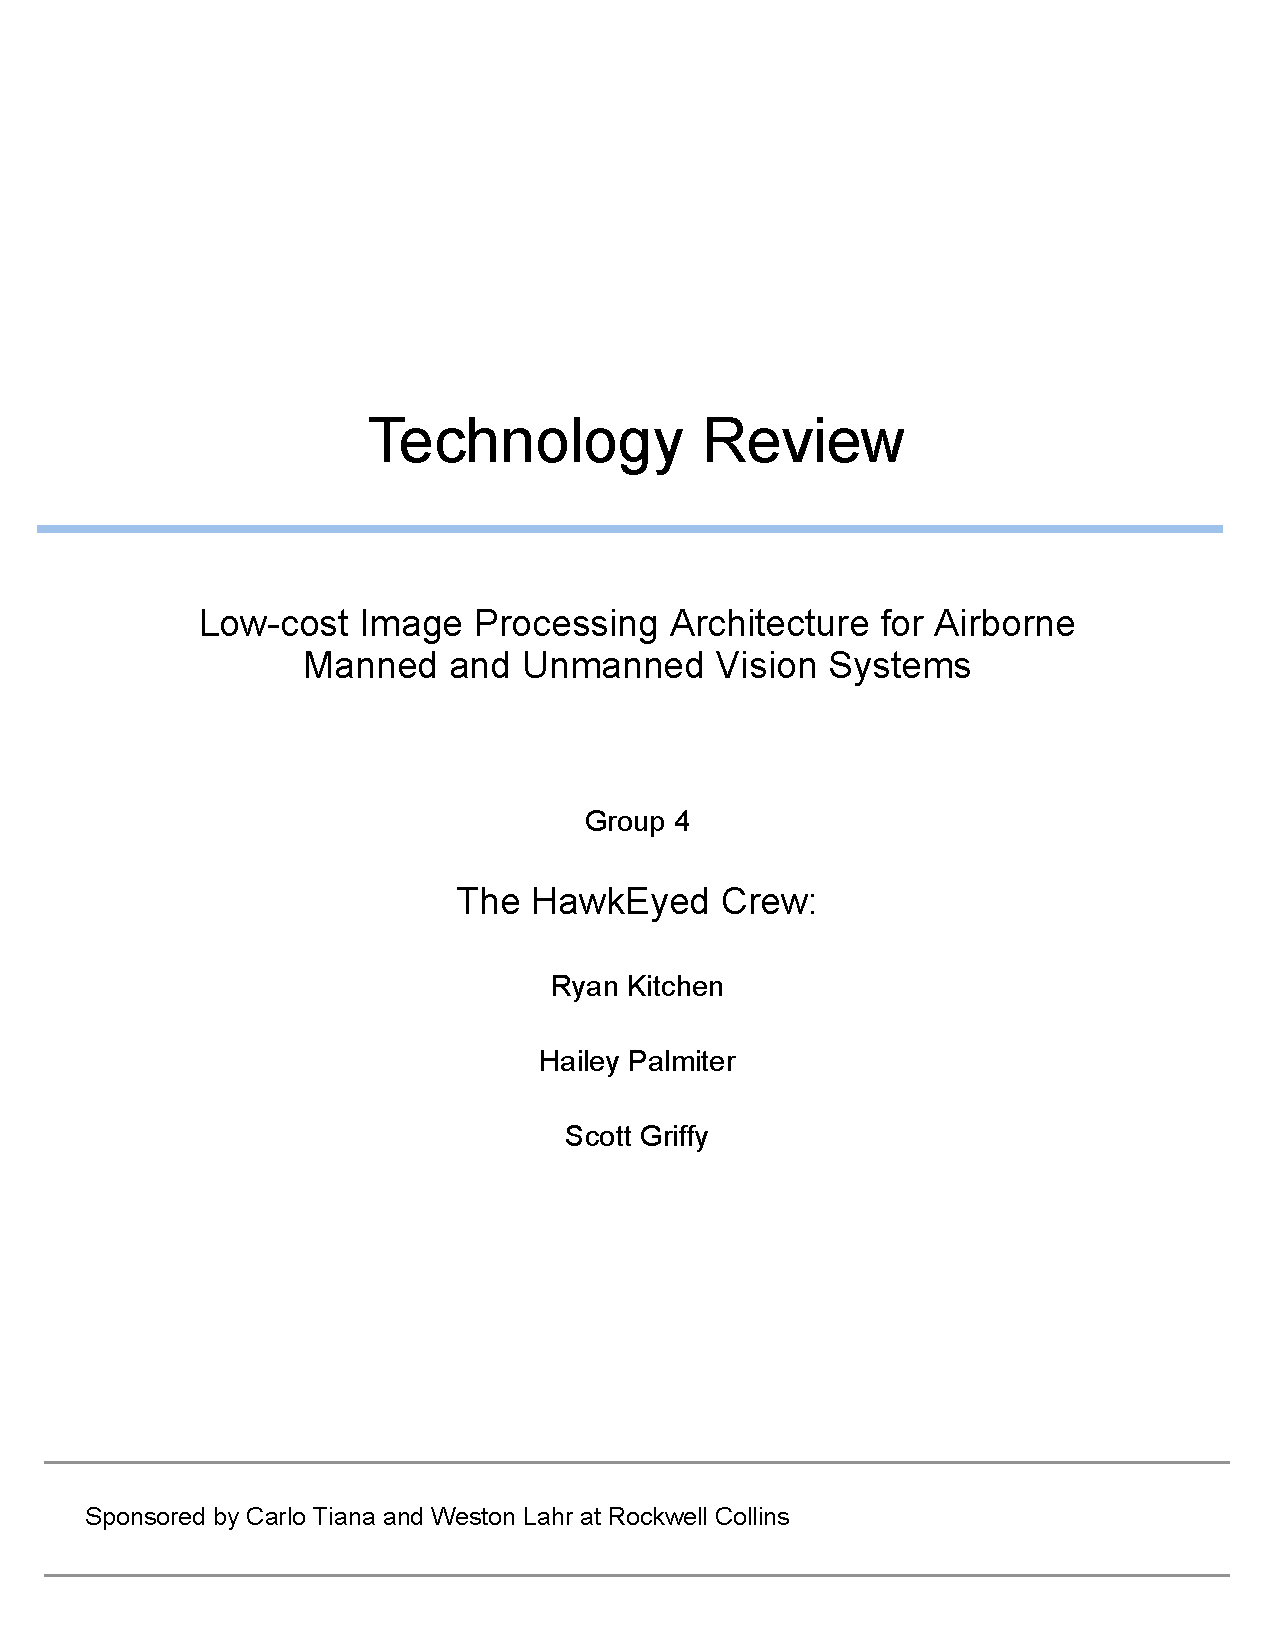
\includepdf[pages=-, frame]{documents/TechReview.pdf}
\subsection{Technology Changes}
\subsubsection{Camera Interface}
For our camera interface we ended up using the USB 3.0 camera setup. This made our code simple, but did require us to work with a USB 3.0 expansion card which had trouble supplying the necessary power to the cameras, requiring the camera's power supplies to be connected while in use.
\subsubsection{Video Subsystem}
For our video software subsystem, we ended up using a different system entirely: CUDA. We talked about OpenCV's performance issues in the Technology Review and they ended up constraining us too much. OpenCV was great for getting a simple program working, but it only ran at around 14 frames per second which was not viable. Writing lower level code in CUDA kernels and using the CUDA API allowed us to take more control over the memory in the TX1 resulting in higher frame rate.
\subsubsection{Image Processing}
We ended up using the on-board GPU for our image processing which is what we thought we were going to use. It was the best option because it was the simplest to code and investigate and it supposedly would meet the requirements, so we had no reason to believe it wouldn't be capable for the project and if it failed we wouldn't have wasted much time.
\subsubsection{Demo Interface}
In our technology review, we discused a lot of software that we thought we might use to display the output of our camera system and decided to use OpenCV to create the project. We ended up using OpenGL instead. Our discussion of the benefits and drawbacks of OpenCV vs OpenGL in the technology review show why we eventually made the switch. The OpenCV GUI ended up being too slow compared to OpenGL. This was because of the benefit we list in OpenGL, saying that it was powerful. We had full control over the buffers that were send to the window for rendering, which allowed us to employ memory mapping magic to reduce the number of memory copies and thus achieve the latency and framerate required for the project. While this was more expensive in terms of coding hours, it ended up being necessary for the project. Though attempting to use OpenCV was a worthwhile effort to learn more about our development environment quickly.

	
\section{Weekly Blog Posts}

	\subsection{Fall Term 2015}
	
	\subsection{Winter Term 2016}
	
	\subsection{Spring Term 2016}

\newpage	
\section{Final Poster}
\begin{figure}[!ht] 
	\centering
	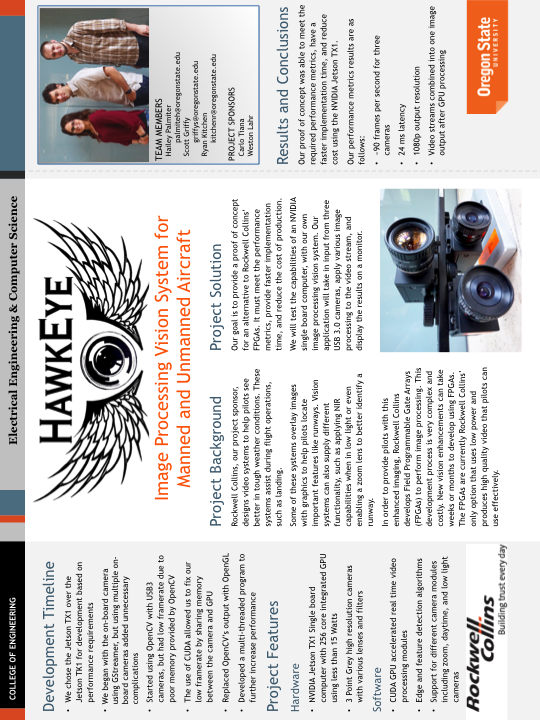
\includegraphics[width=\textwidth,height=\textheight,keepaspectratio]{images/HawkEye_Poster.png}  
	\end{figure}

\section{Project Documentation}

\section{Discovery of New Technologies}

\section{Personal Experiences}

	\subsection{Hailey Palmiter}
	
	\subsection{Scott Griffy}
	
	\subsection{Ryan Kitchen}
	
%Appendix 1 and 2
   
\end{document}
   
